\chapter{Unit roots, spurious regression and cointegration}
\label{cap:ur}

\section{Deterministic versus stochastic trend}
Two series can ``go up'' for very different reasons.
\begin{itemize}[leftmargin=1.4em]
\item \textbf{Deterministic trend}: $y_t=a+bt+\text{(stationary)}$. Deviations from the line are temporary. Removing the trend makes the series stationary.
\item \textbf{Stochastic trend} (unit root): $y_t=y_{t-1}+\varepsilon_t$. Shocks are permanent. Removing a line does \emph{not} solve it; you must difference.
\end{itemize}
Treating one as if it were the other leads to serious forecasting and inference errors.

\section{The augmented Dickey--Fuller (ADF) test}
We estimate
\[
\Delta y_t=\alpha+\gamma\,y_{t-1}+\sum_{j=1}^{p}\delta_j\Delta y_{t-j}+e_t,
\]
and test $H_0:\gamma=0$ (there is a unit root) against $\gamma<0$ (stationary). The extra lags serve to whiten the residuals.

\begin{atencao}[ADF pitfalls]
\begin{itemize}[leftmargin=1.2em]
\item \textbf{The t statistic follows neither the t nor the normal distribution}. The critical values are the Dickey--Fuller ones, more negative (for example, about $-2.86$ at 5\% with a constant). Comparing with $-1.96$ rejects too often.
\item \textbf{The deterministic terms matter}: without constant, with constant or with trend, the critical values change and the wrong choice distorts the test.
\item \textbf{Low power}: the test has difficulty telling a unit root from a root close to 1 (for example, $\phi=0.98$) in moderate samples.
\item \textbf{KPSS reverses the null hypothesis} (the null is stationarity). Using both together is common practice: ADF rejects and KPSS does not reject $\Rightarrow$ evidence in favor of stationarity.
\end{itemize}
\end{atencao}

\begin{simulacao}[Checked by simulation]
In a 300-point random walk, the ADF p-value was $0.50$ (does not reject the unit root, correct). In white noise, the p-value was $\approx10^{-29}$ (strongly rejects, correct).
\end{simulacao}

\section{Spurious regression}
Regressing an integrated series on another, independent of it, produces ``significant'' coefficients with absurd frequency.

\begin{simulacao}[Checked by simulation]
I simulated 1000 pairs of \emph{independent} random walks with 200 observations each, ran OLS of one on the other and tested the slope at 5\%. The t test rejected the null of zero slope in \textbf{83.6\%} of the cases, instead of the expected 5\%.
\end{simulacao}

\begin{center}
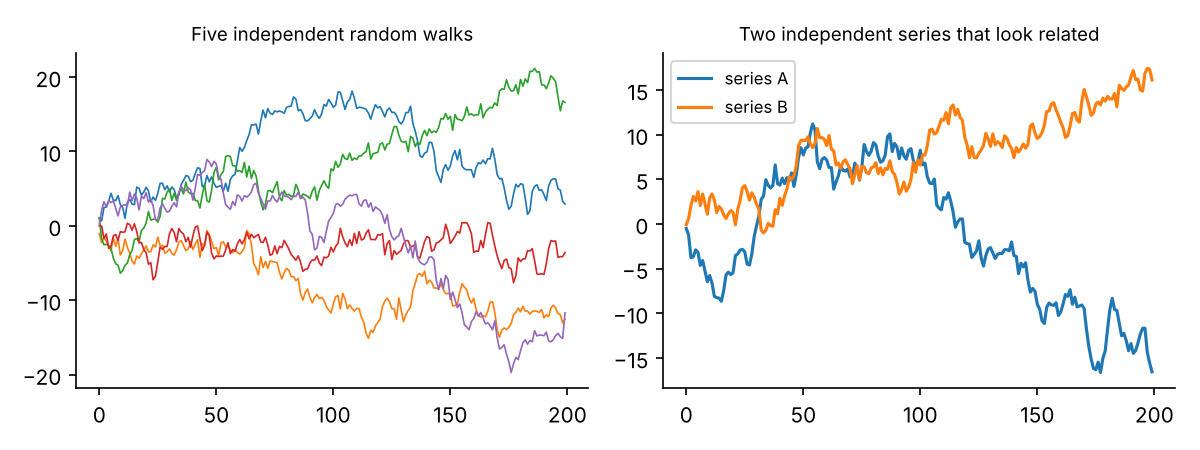
\includegraphics[width=0.9\textwidth]{fig/espuria.png}\\
\small Left: five independent random walks, which seem to have trends of their own. Right: two independent series that, by chance, look related.
\end{center}

\textbf{Practical rules}: (i) never run OLS on levels of series with a unit root without investigating cointegration; (ii) a classic warning sign is a high $R^2$ with strongly autocorrelated residuals (Durbin--Watson statistic close to 0); (iii) if there is no cointegration, work with the differenced series.

\section{Cointegration}
Two $I(1)$ series are \textbf{cointegrated} if some linear combination of them is stationary. They can drift apart in the short run, but a force brings them back (a long-run equilibrium).

\begin{intuicao}[The drunk and the dog]
Two independent random walks are like a drunk and a dog on the loose: each goes wherever it wants. Cointegration is the drunk with the dog on a leash: both wander aimlessly, but the distance between them is bounded.
\end{intuicao}

\begin{center}
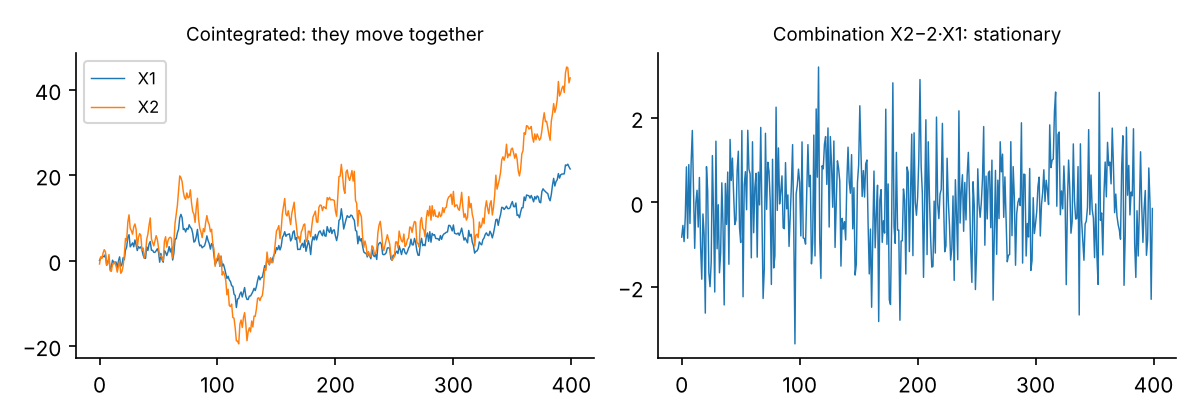
\includegraphics[width=0.9\textwidth]{fig/cointegracao.png}\\
\small $X_1=w+\text{noise}$ and $X_2=2w+\text{noise}$, with $w$ a random walk. Each series is nonstationary, but $X_2-2X_1$ is stationary.
\end{center}

\textbf{Engle--Granger test} (two steps): (1) regress one series on the other; (2) apply ADF to the residuals, using \emph{specific} critical values for estimated residuals (more demanding than those of the ordinary ADF). The multivariate alternative is the Johansen test, which identifies how many cointegrating relations exist.

\begin{simulacao}[Checked by simulation]
With 200 observations, I repeated 500 times. For cointegrated pairs, the Engle--Granger test at 5\% rejected ``no cointegration'' in 99.6\% of the simulations. For independent pairs, it rejected in 7.4\% (slightly above the nominal 5\% in moderate samples, but very far from 84\%).
\end{simulacao}

\textbf{Error correction model}: if $y_t$ and $x_t$ are cointegrated, $\Delta y_t=\alpha(y_{t-1}-\beta x_{t-1})+\gamma\Delta x_t+e_t$, with $\alpha<0$ measuring the speed at which the economy returns to equilibrium.

\begin{exercicio}
A regression between two price series in levels gives $R^2=0.95$ and Durbin--Watson of $0.1$. What should be done before trusting this result?
\end{exercicio}
\sol{The pattern (high $R^2$, very low DW) is typical of spurious regression. Test for a unit root in each series; if both are $I(1)$, test for cointegration (Engle--Granger or Johansen). Without cointegration, the regression in levels has no interpretation and the correct approach is to model the differences. With cointegration, use an error correction model.}
